\documentclass[main]{subfiles}
\begin{document}

%@@@@@@@@@@@@@@@@@@@@@@@@@@@@@@
% Main Topics: Plasticity and Learning 08.11.2018
% Lecturer: Daniel Kiper
% author: Vanessa Leite - base document from benelot/eth-intro-to-neuroinformatics-summary

\section{Plasticity and Learning}
\subsection{Learning and Memory}
\begin{itemize}[noitemsep,nolistsep]
	\item Learning is the acquisition of new information or knowledge.
	\item Memory is the retention of learned information.
	\item The brain has a more complex configuration than given by genes.
	\item There is lots of room for learning (and also need).
	\item Only brain area responsibility and cortex thickness (6 layers) are genetically fixed. But even that can sometimes change later on.
\end{itemize}

\subsubsection{Types of Memory}
\begin{itemize}[noitemsep,nolistsep]
	\item Declarative memory (facts, events)
	\item Non-declarative memory
	\item Procedural memory (skill, habits)
	\item Emotional responses
\end{itemize}

\subsubsection{Connections to Synapses}
\begin{itemize}[noitemsep,nolistsep]
	\item Neurons communicate via AP and are interconnected via synapses.
	\item Information is represented by distributed activity.
	\item Learning and memory is based on changes in synaptic connections.
	\item Synapses get formated, retracted.
	\item Synapse efficacies/plasticity can change.
\end{itemize}

\subsection{Plasticity}
\begin{itemize}[noitemsep,nolistsep]
	\item Modification of postsynaptic potentials (PSPs) evoked by presynaptic spikes.
	\item A: Postsynaptic response triggered by a weak test pulse.
	\item B: Strong stimulation triggers postsynaptic firing.
	\item C: A later test pulse evokes a larger postsynaptic response than initially.
\end{itemize}

\begin{figure}[H]
	\centering
	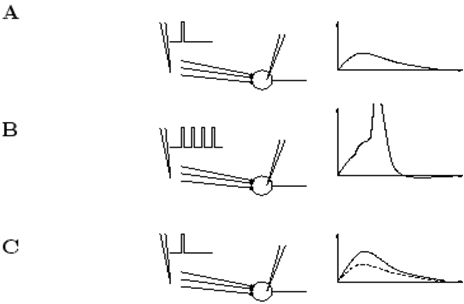
\includegraphics[scale=0.5]{plasticity.png}
\end{figure}

\subsubsection{Parameters that define synapse strengths}
\begin{itemize}[noitemsep,nolistsep]
	\item Neurotransmitter and receptor type
	\item Position of synapse
	\item Availability of vesicles
	\item Re-uptake of transmitters
	\item Neuromodulators, such as dopamine
	\item Postsynaptic cellular processes (such as more or less receptors)
	\item Pre/postsynaptic firing
\end{itemize}

\subsubsection{Models of Synaptic Plasticity}
\begin{itemize}[noitemsep,nolistsep]
	\item There is also non synaptic plasticity, such as dendrite strength, excitability of neurons, isolation of axons.
	\item Phenomenological models show input-output relationships between activity and plasticity.
	\item Biophysical models tell what processes are involved.
	\item Hebb's Postulate: ``When an axon of cell A is near enough to excite cell B or repeatedly or persistently takes part in firing it, some growth process or metabolic change takes place in one or both cells, such that A's efficiency, as one of the cells firing B, is increased''
\end{itemize}

\subsection{Pavlovian Conditioning}
\begin{figure}
	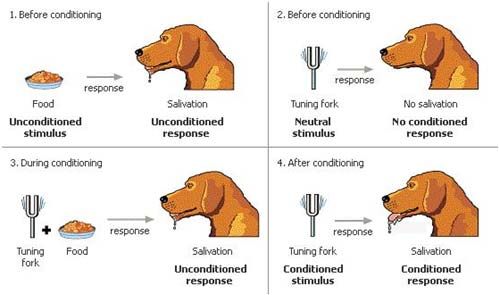
\includegraphics[width=0.9\textwidth]{pavlovian-conditioning.png}
\end{figure}

\subsection{Hebbian Learning}
\begin{itemize}[noitemsep,nolistsep]
	\item Learning based on correlations between pre- and postsynaptic firing.
	\item Uses only variables locally available at the synapse.
	\item Expressed in a rate-based model: $\Delta w_{ij}\propto v_i\cdot v_j$.
	\item Only weight increases, potentiation modeled.
	\item It will lead to instability because of positive feedback loops.
	\item Other rules can be added for weight reduction (depression) and normalization (Oja, BCM).
	\item Hebb's postulate implies constraints for synaptic learning:
	\subitem Direction of information flow (forward).
	\subitem Global effects arise from local learning.
	\subitem Variables are action potentials, synapse weights (efficacy) and neuromodulator/calcium concentration (locally).
\end{itemize}

\subsection{NMDA Synapse}
\begin{figure}[H]
	\centering
	\begin{subfigure}[b]{0.5\textwidth}
    	\centering
		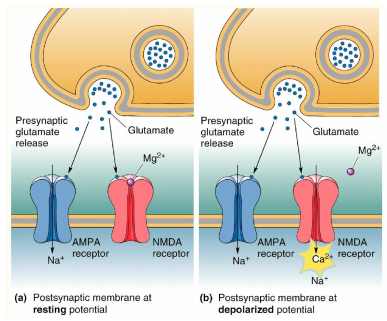
\includegraphics[width=\textwidth]{NMDA_receptor_01.png}
	\end{subfigure}%
	~
	\begin{subfigure}[b]{0.5\textwidth}
		\centering
		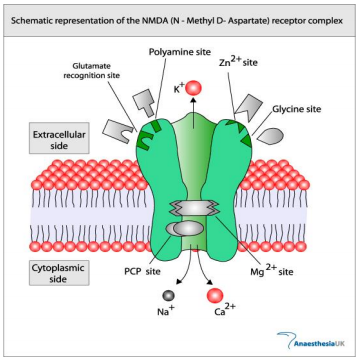
\includegraphics[width=\textwidth]{NMDA_receptor_02.png}
	\end{subfigure}
\end{figure}
\begin{itemize}[noitemsep,nolistsep]
	\item Can act as a coincidence detector for pre- and postsynaptic firing.
	\subitem Backpropagating action potentials.
	\subitem Depolarization from other synapses.
	\item Calcium influx is crucial for plasticity.
	\item Strong NMDA receptor activation gives potentiation.
	\item Weak NMDA receptor activation gives depression.
\end{itemize}
\subsubsection{Potentiation with NMDA}
\begin{itemize}[noitemsep,nolistsep]
	\item Phosphorylation of AMPA receptors makes the synapse stronger.
	\item Synthesis of new AMPA (but not NMDA) receptors.
	\item Transport of AMPA receptors to membrane.
	\item Release probability or quantity of the presynapse can be improved.
\end{itemize}

\subsection{Short-term plasticity (STP)}
\begin{figure}[H]
	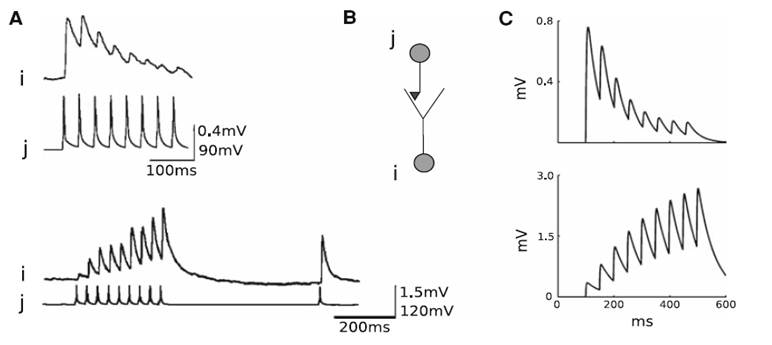
\includegraphics[width=0.8\textwidth]{STP.png}
\end{figure}
\begin{itemize}[noitemsep,nolistsep]
	\item A neuron j fires several times, neuron i fires as well and the spike size is increased(the higher the spike, the more efficient the neuron), but decreases after a short time (caused by loss of vesicles).
	\item Effect goes away in order of milliseconds to seconds.
	\item Short term depression is a safety mechanism.
\end{itemize}

\subsection{Long-term potentiation (LTP)}
\begin{itemize}[noitemsep,nolistsep]
	\item The hippocampus is involved in transferring from short to long term memory.
	\item Tetanus stimulus, strong, high frequent stimulation are required.
	\item A pre- and postsynaptic depolarization at the same time is needed.
	\item Voltage clamp during tetanus prevents LTP from happening.
	\item LTP is cooperative, many weak synapse stimulations give also some effect.
	\item LTP needs a simultaneous depolarization beyond a threshold.
	\item LTP is input specific and can enhance the synaptic effectiveness of a synapse without affecting other synapses in the same cell. This increases the storage capacity of individual neurons.
	\item LTP is associative, weak stimulation in pathways coupled with strong simulation in other pathways can induce LTP.
	\item Stimuli must be delivered at high frequency, because the post-synaptic cell must be depolarized past a certain threshold for LTP.
	\item LTP has a transient early phase ($1-3$ hours), followed by a consolidate later phase ($\geq 24$ hours). The early phase doesn't need new protein synthesis. The later phase needs protein and RNA synthesis for new presynaptic active zones and postsynaptic receptors.
\end{itemize}

\subsection{Long-term depression (LTD)}
\begin{itemize}[noitemsep,nolistsep]
	\item Weakening of the synapse.
\end{itemize}

\subsection{Spike-timing dependent Plasticity (STDP)}
\begin{itemize}[noitemsep,nolistsep]
	\item Not only correlation but also timing of spikes is important.
	\item NMDA receptors and backpropagating action potential creates this timing-dependence of plasticity.
	\item Sign of plasticity is determined by local calcium concentration.
	\item Postsynaptic spike travels back to the dendritic tree and activates voltage-dependent Ca channels.
	\item Presynaptic activity can allow Ca influx through NMDA channels, if the postsynaptic part is sufficiently depolarized.
	\item If pre-spike is soon afterwards followed by post-spike, NMDA-R activity is supralinearly enhanced by depolarization due to backpropagating spike.
\end{itemize}

\begin{figure}[H]
	\centering
	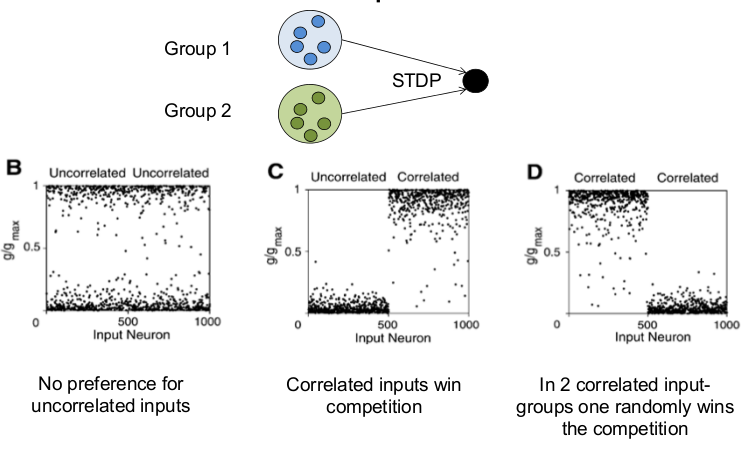
\includegraphics[width=0.8\textwidth]{STDP-consequences.png}
\end{figure}

\begin{figure}[H]
	\centering
	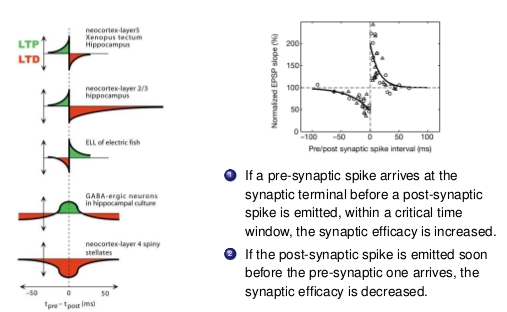
\includegraphics[scale=1]{8_1.jpg}
\end{figure} 

\subsubsection{Functional consequences of STDP}
\begin{itemize}[noitemsep,nolistsep]
	\item Rate normalization, temporal coding, reduced latency, prediction and conditioning.
	\item Only one direction can get stronger, no positive feedback can occur.
	\item STDP can become a simple temporal pattern detector and already fire on the beginning of such a pattern.
	\item Stimulation frequency has an effect on STDP.
	\item Dopamine can extend the LTP timing window or even convert LTD to LTP. Dopamine floats around the cells.
	\item LTP is blocked by AP5. Behavioral success and LTP are correlated.
\end{itemize}

\subsection{Factors that influence plasticity}
\begin{itemize}[noitemsep,nolistsep]
	\item Different plasticity in different brain areas.
	\item Diversity of neuron and synapse types.
	\item Large number of control parameters for plasticity experiments.
	\item Influence of neuromodulators, calcium, drugs, proteins.
	\item Long term vs. short term effects.
	\item Unlikely that a single model explains all plasticity effects found in biology.
\end{itemize}



\end{document}
